\chapter{Overview}\label{cap:overview}

Para a construção do time de robôs autônomos para competir na categoria \textit{Small Size League}  da RoboCup 2017 foi escolhido como módulo de controle uma placa STM32F4-Discovery (mostrada na Figura~\ref{fig:modulo_controle}), comercializada pela STMicroelectronics, contendo o microcontrolador STM32F407VG (de arquitetura ARM32 Cortex M4), responsável por realizar as operações lógicas do robô, servindo como cérebro do sistema eletrônico.

\begin{figure}[H]
  \centering
  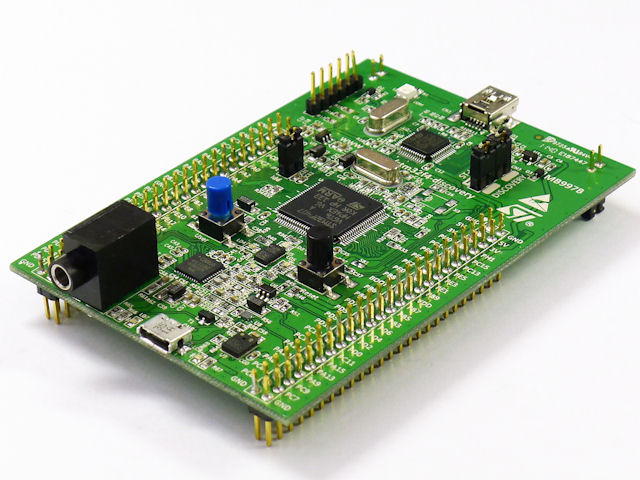
\includegraphics[height=8cm]{modulo_controle}
  \caption{Módulo de Controle}\label{fig:modulo_controle}
\end{figure}

O módulo de transmissão, responsável pela comunicação entre a inteligência e o módulo de controle do robô, consiste em uma placa comercial contendo o chip NRF24L01P e os periféricos necessários para o seu uso (ver Figura~\ref{fig:modulo_transmissao}). O módulo é ligado ao módulo de controle do robô através da placa mãe e se comunica com este utilizando o protocolo SPI (\textit{Serial Peripheral Interface}). Para fazer a comunicação com a inteligência, o módulo se comunica com outro igual ligado ao computador onde a inteligência está sendo executada utilizando uma frequência na faixa de 2,4 GHz. Para a comunicação entre dois módulos, o chip utiliza um protocolo próprio chamado Enhanced ShockBurst™, uma camada de vínculo de dados (camada de protocolo que lida com a entrada e saída de sequências de bits no meio físico, escondendo das camadas superiores o hardware subjacente e lidando com os pacotes perdidos e os pacotes duplicados) que permite envio de pacotes de confirmação sem a necessidade de receptor e transmissor inverterem seus modos de funcionamento (funcionalidade chamada \textit{Auto Acknowledgement}).
Isso permite ganhar tempo no envio das informações que a inteligência precisa.

\begin{figure}[H]
  \centering
  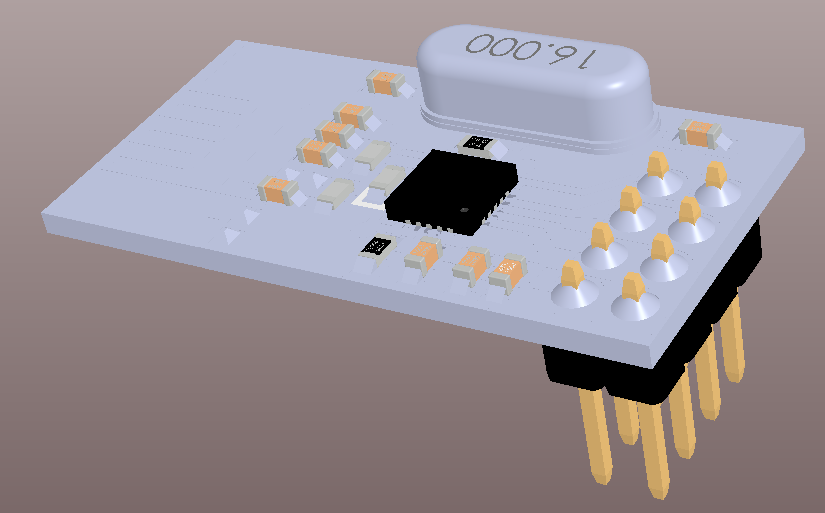
\includegraphics[height=8cm]{modulo_transmissao}
  \caption{Módulo de Transmissão}\label{fig:modulo_transmissao}
\end{figure}

Devido ao fato de o módulo de transmissão escolhido ser controlado por interface SPI, fez-se necessário aprender a utilizar a interface SPI do módulo de controle(STM32F4-Discovery), o que levou à confecção de uma  biblioteca de funções para comunicação SPI para o microcontrolador STM32F407VG.

% Ramificação constante ou taxa constante

% vim: tw=80 et ts=2 sw=2 sts=2 ft=tex spelllang=pt_br,en
